\providecommand{\main}{../../..}
\documentclass[\main/main.tex]{subfiles}
\begin{document}

\subsection{Exercise 14}
The following problem is given:

\begin{align*}
  \min f_1(x) = x_1^2 + x_2^2 - 2x_1 \\
  \min f_2(x) = -x_2                 \\
  x_1^2 + 4x^2_2 & \leq 8            \\
  x_1 - 2x_2     & \geq 0
\end{align*}


Identify the utopy point and determine the preferable solution between $A' = (-1,0)$, $B'=(\sfrac{-3}{4}, \sfrac{-1}{2})$ and $C' = (1, -1)$ using the Manhattan distance.

\subsection{Resolution exercise 14}
The minima for the first function is the center, $\bmx = (1,0)$, $f_1 = -1$.

The minima for the second objective function is $\bmx=(2,1)$, $f_2 = -1$.

The minimum distance via the Manhattan distance is $B$.

\begin{figure}
  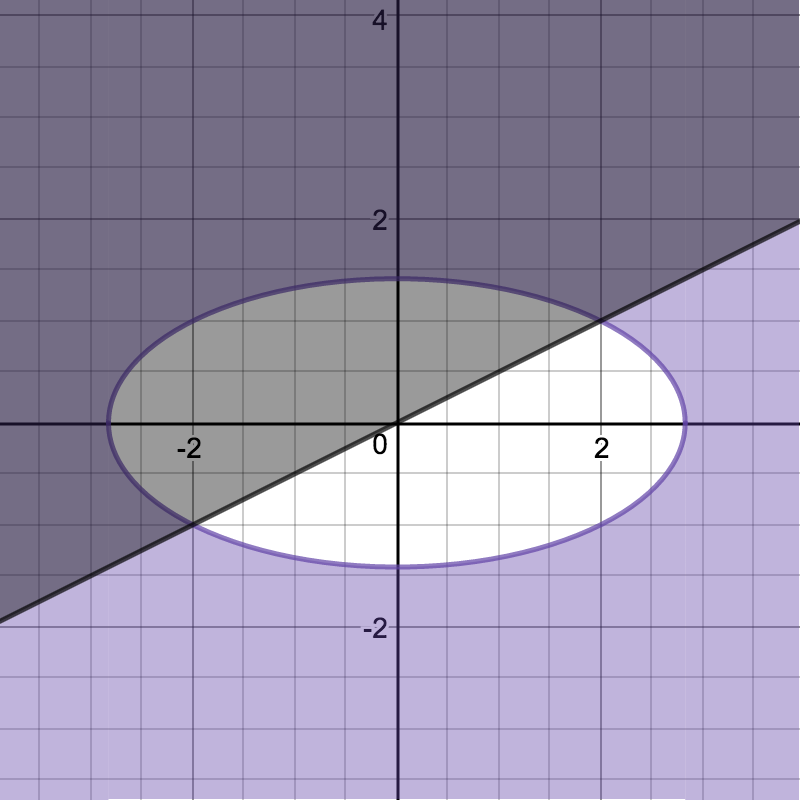
\includegraphics[width=0.4\textwidth]{es14-maut}
\end{figure}


\end{document}